\documentclass{standalone}
\usepackage{tikz}
\usetikzlibrary{patterns, positioning}
\usetikzlibrary{shapes.misc}
\usepackage[outline]{contour}
\contourlength{1.5pt} 
\usepackage[sfdefault]{ClearSans} %% option 'sfdefault' activates Clear Sans as the default text font
\usepackage[T1]{fontenc}

\begin{document}
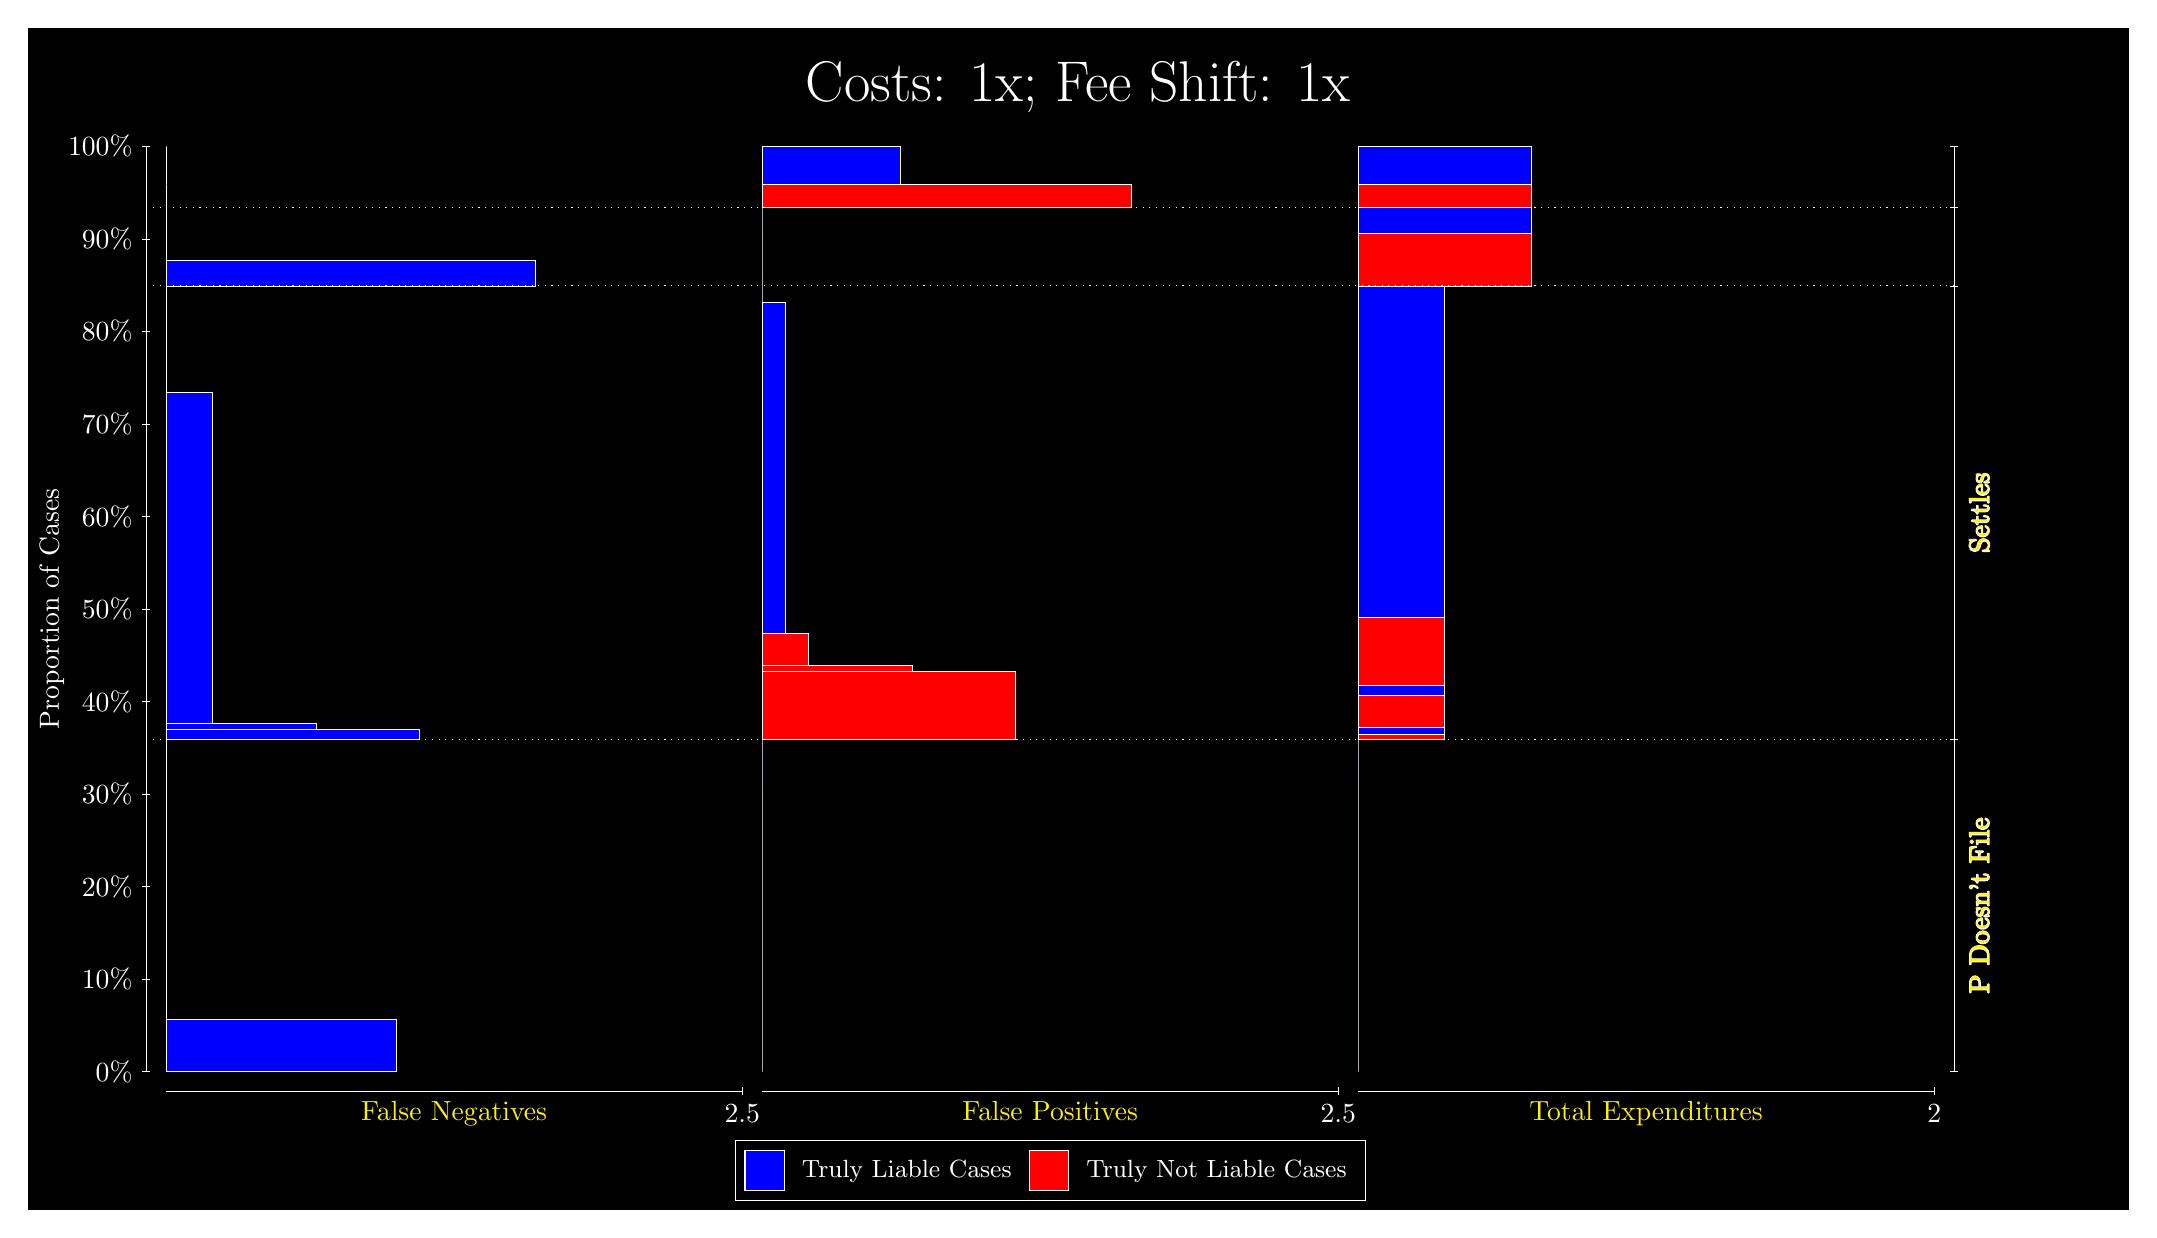
\begin{tikzpicture}
\draw[fill=black] (0,0) rectangle (26.667,15);
\draw[text=white] (0,13.5) rectangle (26.667,15) node[midway] {\huge Costs: 1x; Fee Shift: 1x};
\draw[white, very thin] (1.5,1.75) -- (1.5,13.5);
\node[rotate=90, text=white, anchor=center] at (0.3, 7.625) {Proportion of Cases};
\draw[white, very thin] (1.45,1.75) -- (1.55,1.75);
\node[text=white, anchor=east] at (1.45, 1.75) {0\%};
\draw[white, very thin] (1.45,2.925) -- (1.55,2.925);
\node[text=white, anchor=east] at (1.45, 2.925) {10\%};
\draw[white, very thin] (1.45,4.1) -- (1.55,4.1);
\node[text=white, anchor=east] at (1.45, 4.1) {20\%};
\draw[white, very thin] (1.45,5.275) -- (1.55,5.275);
\node[text=white, anchor=east] at (1.45, 5.275) {30\%};
\draw[white, very thin] (1.45,6.45) -- (1.55,6.45);
\node[text=white, anchor=east] at (1.45, 6.45) {40\%};
\draw[white, very thin] (1.45,7.625) -- (1.55,7.625);
\node[text=white, anchor=east] at (1.45, 7.625) {50\%};
\draw[white, very thin] (1.45,8.8) -- (1.55,8.8);
\node[text=white, anchor=east] at (1.45, 8.8) {60\%};
\draw[white, very thin] (1.45,9.975) -- (1.55,9.975);
\node[text=white, anchor=east] at (1.45, 9.975) {70\%};
\draw[white, very thin] (1.45,11.15) -- (1.55,11.15);
\node[text=white, anchor=east] at (1.45, 11.15) {80\%};
\draw[white, very thin] (1.45,12.325) -- (1.55,12.325);
\node[text=white, anchor=east] at (1.45, 12.325) {90\%};
\draw[white, very thin] (1.45,13.5) -- (1.55,13.5);
\node[text=white, anchor=east] at (1.45, 13.5) {100\%};

\draw[white, very thin] (24.457,1.75) -- (24.457,13.5);
\draw[white, very thin] (24.407,1.75) -- (24.507,1.75);
\node[anchor=west] at (24.407, 1.75) {};
\draw[white, very thin] (24.407,5.9665) -- (24.507,5.9665);
\node[anchor=west] at (24.407, 5.9665) {};
\draw[white, very thin] (24.407,11.727) -- (24.507,11.727);
\node[anchor=west] at (24.407, 11.727) {};
\draw[white, very thin] (24.407,12.721) -- (24.507,12.721);
\node[anchor=west] at (24.407, 12.721) {};
\draw[white, very thin] (24.407,13.5) -- (24.507,13.5);
\node[anchor=west] at (24.407, 13.5) {};

\draw[white, very thin, fill=blue] (1.75,1.75) rectangle (4.6775,2.4112);
\draw[white, very thin, fill=red] (1.75,2.4112) rectangle (1.75,5.9665);
\draw[white, very thin, fill=blue] (1.75,5.9665) rectangle (4.9703,6.0903);
\draw[white, very thin, fill=blue] (1.75,6.0903) rectangle (3.6529,6.1713);
\draw[white, very thin, fill=blue] (1.75,6.1713) rectangle (2.3355,10.376);
\draw[white, very thin, fill=red] (1.75,10.376) rectangle (1.75,11.727);
\draw[white, very thin, fill=blue] (1.75,11.727) rectangle (6.4341,12.05);
\draw[white, very thin, fill=red] (1.75,12.05) rectangle (1.75,12.721);
\draw[white, very thin, fill=red] (1.75,12.721) rectangle (1.75,13.018);
\draw[white, very thin, fill=blue] (1.75,13.018) rectangle (1.75,13.5);
\draw[white, very thin, fill=red] (9.3189,1.75) rectangle (9.3189,5.3052);
\draw[white, very thin, fill=blue] (9.3189,5.3052) rectangle (9.3189,5.9665);
\draw[white, very thin, fill=red] (9.3189,5.9665) rectangle (12.539,6.8304);
\draw[white, very thin, fill=red] (9.3189,6.8304) rectangle (11.222,6.9032);
\draw[white, very thin, fill=red] (9.3189,6.9032) rectangle (9.9044,7.3175);
\draw[white, very thin, fill=blue] (9.3189,7.3175) rectangle (9.6116,11.522);
\draw[white, very thin, fill=blue] (9.3189,11.522) rectangle (9.3189,11.727);
\draw[white, very thin, fill=red] (9.3189,11.727) rectangle (9.3189,12.398);
\draw[white, very thin, fill=blue] (9.3189,12.398) rectangle (9.3189,12.721);
\draw[white, very thin, fill=red] (9.3189,12.721) rectangle (14.003,13.018);
\draw[white, very thin, fill=blue] (9.3189,13.018) rectangle (11.075,13.5);
\draw[white, very thin, fill=red] (16.888,1.75) rectangle (16.888,5.3052);
\draw[white, very thin, fill=blue] (16.888,5.3052) rectangle (16.888,5.9665);
\draw[white, very thin, fill=red] (16.888,5.9665) rectangle (17.986,6.0393);
\draw[white, very thin, fill=blue] (16.888,6.0393) rectangle (17.986,6.1202);
\draw[white, very thin, fill=red] (16.888,6.1202) rectangle (17.986,6.5344);
\draw[white, very thin, fill=blue] (16.888,6.5344) rectangle (17.986,6.6583);
\draw[white, very thin, fill=red] (16.888,6.6583) rectangle (17.986,7.5223);
\draw[white, very thin, fill=blue] (16.888,7.5223) rectangle (17.986,11.727);
\draw[white, very thin, fill=red] (16.888,11.727) rectangle (19.083,12.398);
\draw[white, very thin, fill=blue] (16.888,12.398) rectangle (19.083,12.721);
\draw[white, very thin, fill=red] (16.888,12.721) rectangle (19.083,13.018);
\draw[white, very thin, fill=blue] (16.888,13.018) rectangle (19.083,13.5);
\draw[white, dotted] (1.5,5.9665) -- (24.457,5.9665);
\draw[white, dotted] (1.5,11.727) -- (24.457,11.727);
\draw[white, dotted] (1.5,12.721) -- (24.457,12.721);
\draw[white, very thin] (1.75,1.5) -- (9.0689,1.5);
\node[text=yellow, anchor=north] at (5.4094, 1.5) {False Negatives};
\draw[white, very thin] (9.0689,1.45) -- (9.0689,1.55);
\node[text=white, anchor=north] at (9.0689, 1.45) {2.5};

\draw[white, very thin] (9.3189,1.5) -- (16.638,1.5);
\node[text=yellow, anchor=north] at (12.978, 1.5) {False Positives};
\draw[white, very thin] (16.638,1.45) -- (16.638,1.55);
\node[text=white, anchor=north] at (16.638, 1.45) {2.5};

\draw[white, very thin] (16.888,1.5) -- (24.207,1.5);
\node[text=yellow, anchor=north] at (20.547, 1.5) {Total Expenditures};
\draw[white, very thin] (24.207,1.45) -- (24.207,1.55);
\node[text=white, anchor=north] at (24.207, 1.45) {2};

\node[text=yellow, centered, rotate=90] at (24.777, 3.8582) {\contour{white}{P Doesn't File}};
\node[text=yellow, centered, rotate=90] at (24.777, 8.8468) {\contour{white}{Settles}};



\draw (12.978300999999998,1.5) node[draw=none] (baseCoordinate) {};
\begin{scope}[align=center]
        \matrix[scale=0.5, draw=white, below=0.5cm of baseCoordinate, nodes={draw}, column sep=0.1cm]{
            \node[rectangle, draw, minimum width=0.5cm, minimum height=0.5cm, fill=blue] {}; &
            \node[draw=none, font=\small, text=white] (B) {Truly Liable Cases}; &
            \node[rectangle, draw, minimum width=0.5cm, minimum height=0.5cm, fill=red] {}; &
            \node[draw=none, font=\small, text=white] (B) {Truly Not Liable Cases}; \\
            };
\end{scope}

\end{tikzpicture}
\end{document}